%%%
\subsection*{Global results}

We have analysed the microbiome temporal variability to extract global properties of the system. As fluctuations in total counts are plagued by systematic errors we worked on temporal variability of relative abundances for each taxon. Our first finding was that, in all cases, changes in relative abundances of taxa follow a ubiquitous pattern known as the fluctuation scaling law\cite{fs} or Taylor's  power law\cite{taylor}, i.e., microbiota of all detected taxa follows $\sigma_i  = V\cdot x_i^{\beta}$, a power law dependence between mean relative abundance $x_i$ and dispersion $\sigma_i$. The law seem to be ubiquitous, spanning even to six orders of magnitude in the observed relative abundances (see Figure \ref{fig:main1}). 

\begin{figure}
	\centering
	\vspace*{-15mm} % Corrects overbox of the figures
	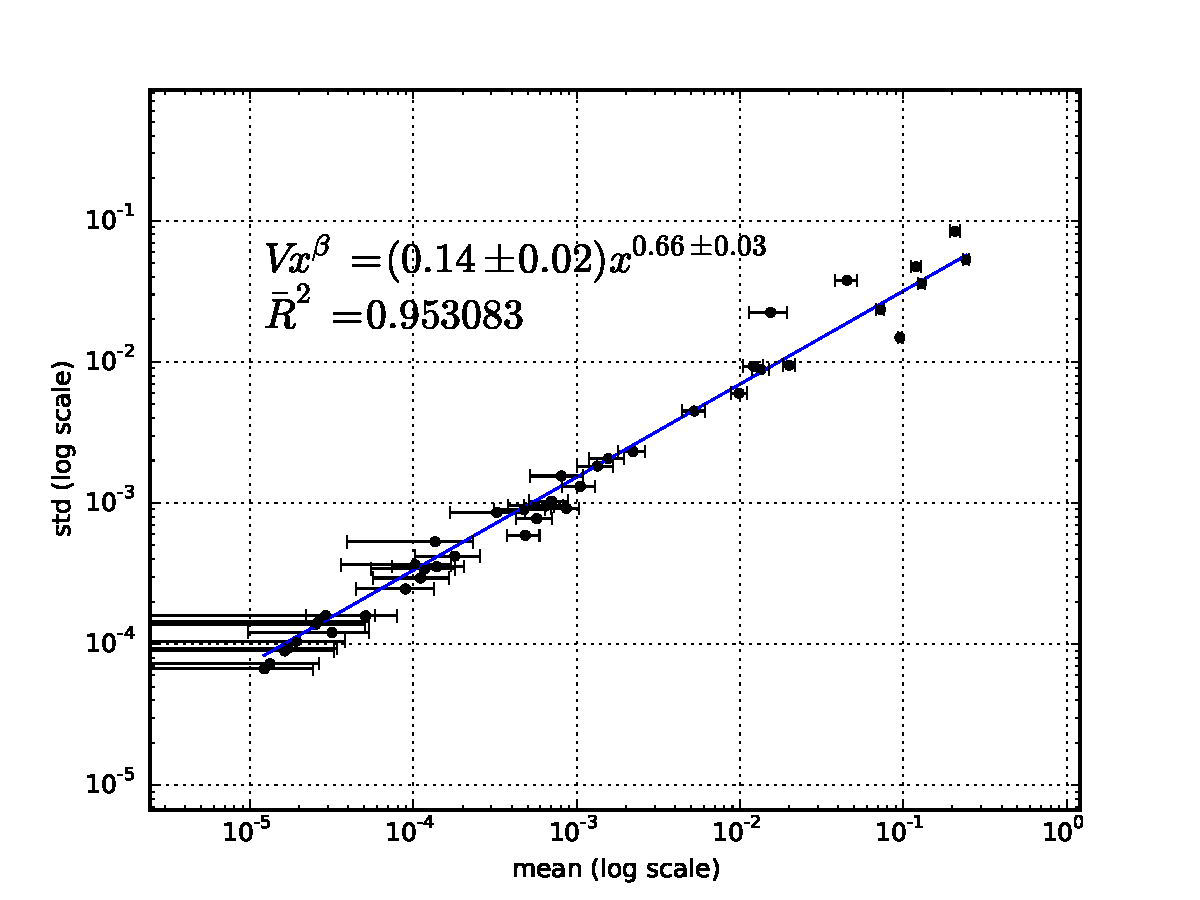
\includegraphics[width=0.8\textwidth]{results/fits/IBS_h_A_amplicons_family_stdVSmean_xWboot_LOG.pdf}
	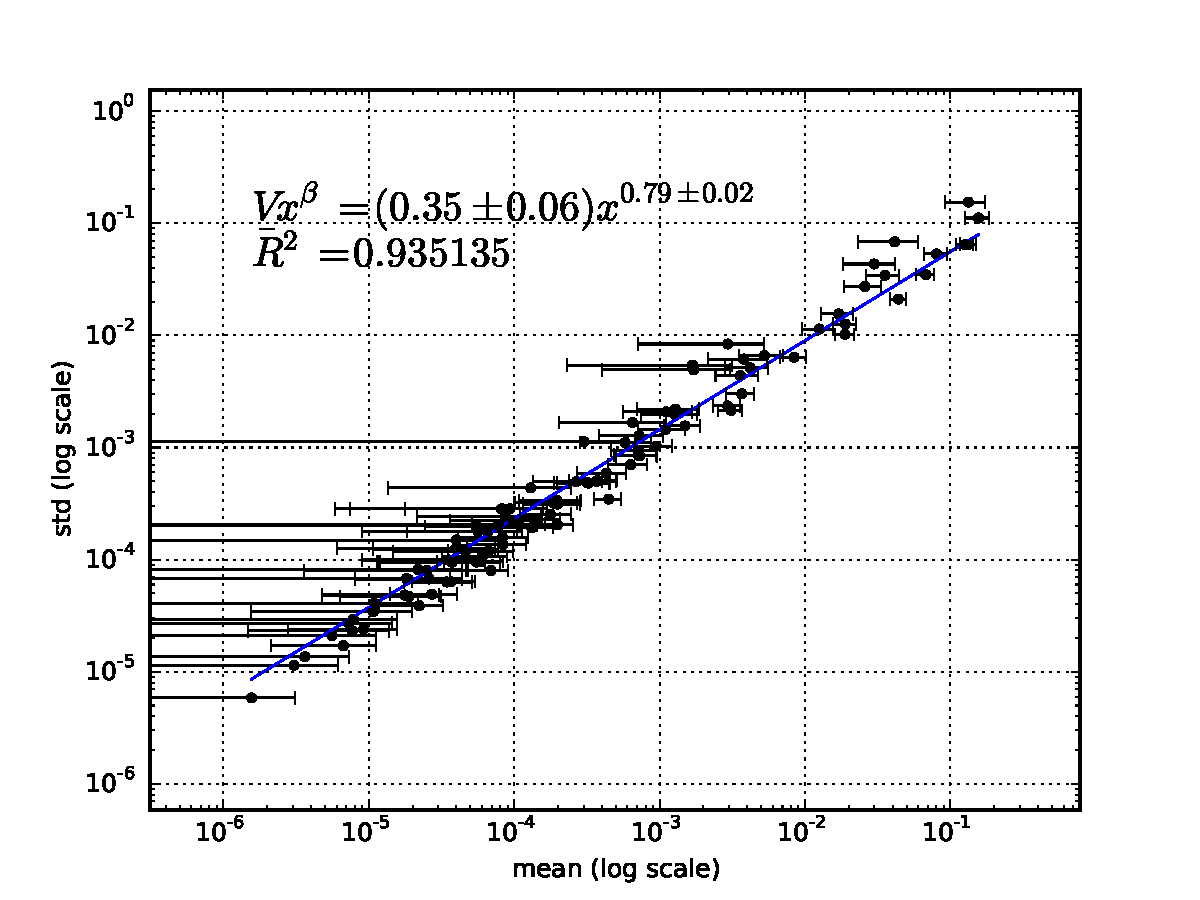
\includegraphics[width=0.8\textwidth]{results/fits/IBS_P2_Metatranscriptores_stdVSmean_xWboot_LOG.pdf}
	\caption{X-weighted power-law fits of the standard deviations versus the mean values for each bacterial genus monitored in time. We show the fit for samples from a healthy subject (top) and from a subject diagnosed with irritable bowel syndrome (bottom), studied in our lab \cite{IBS}. Taylor's power law seems to be ubiquitous, spanning to six orders of magnitude.}
	\label{fig:main1}
\end{figure}

The power law (or scaling) index $\beta$ and the variability $V$ (hereafter Taylor parameters) appear to be correlated with the stability of the community and related with the health status of the host, which we consider the main finding exposed in this article (see Figure \ref{fig:main2}).

\begin{figure}
	\centering
	\includegraphics[width=0.9\textwidth]{results/finalplot11.pdf}
	\caption{Taylor's law parameter space. We have compiled here all the data studied in this work. The coloured circle corresponds to 68\% confidence level (CL) region of healthy individuals in the Taylor parameter space, while dashed line delimites the 98\% CL region. Points with errors place each individual gut microbiome in the Taylor space. Note that the parameters have been standardized (stdev units) to the healthy group in each study for demonstrative and comparative purposes.}
	\label{fig:main2}
\end{figure}

Taylor parameters describing the temporal variability of the gut microbiome in our sampled individuals are shown in Tables \ref{tab:diet} to \ref{tab:LEA}. Our results hint at an ubiquitous behaviour. On the first hand, the variability (which corresponds to the maximum amplitude of fluctuations) is large, which suggests resilient capacity of the microbiota. On the other hand, the scaling index is always smaller than one, which means that more abundant taxa are less volatile than less abundant ones. In addition, Taylor parameters for the microbiome of healthy individuals in different studies are compatible within estimated errors. This enables us to define an area in the Taylor parameter space that we called the \emph{healthy zone}.

\begin{table} 
  \begin{center}
    \begin{tabular}{ccccccc}
	    \hline
		Metadata&V&$\beta$&$\bar{R}^2$&&V$_{st}$&$\beta_{st}$\\
		\hline
		A&$0.26 \pm 0.05$&$0.826 \pm 0.025$&$0.918$&&$3.1 \pm 0.9$&$1.2 \pm 0.6$\\
		A&$0.32 \pm 0.06$&$0.857 \pm 0.025$&$0.924$&&$4.4 \pm 1.1$&$2.0 \pm 0.6$\\
		A&$0.194 \pm 0.033$&$0.813 \pm 0.024$&$0.918$&&$1.9 \pm 0.6$&$0.9 \pm 0.6$\\
		A&$0.24 \pm 0.04$&$0.824 \pm 0.020$&$0.924$&&$2.7 \pm 0.7$&$1.2 \pm 0.5$\\
		A&$0.34 \pm 0.06$&$0.855 \pm 0.024$&$0.931$&&$4.7 \pm 1.1$&$1.9 \pm 0.6$\\
		A&$0.30 \pm 0.05$&$0.847 \pm 0.022$&$0.921$&&$3.9 \pm 1.0$&$1.7 \pm 0.5$\\
		A&$0.133 \pm 0.021$&$0.784 \pm 0.023$&$0.916$&&$0.7 \pm 0.4$&$0.2 \pm 0.6$\\
		A&$0.25 \pm 0.04$&$0.831 \pm 0.024$&$0.929$&&$3.0 \pm 0.8$&$1.4 \pm 0.6$\\
		\hline
		P&$0.23 \pm 0.05$&$0.804 \pm 0.035$&$0.885$&&$2.6 \pm 0.9$&$0.7 \pm 0.8$\\
		P&$0.097 \pm 0.018$&$0.705 \pm 0.031$&$0.891$&&$0.03 \pm 0.34$&$-1.6 \pm 0.7$\\
		P&$0.037 \pm 0.006$&$0.642 \pm 0.025$&$0.881$&&$-1.12 \pm 0.11$&$-3.1 \pm 0.6$\\
		P&$0.118 \pm 0.019$&$0.723 \pm 0.025$&$0.895$&&$0.4 \pm 0.4$&$-1.2 \pm 0.6$\\
		P&$0.17 \pm 0.04$&$0.78 \pm 0.04$&$0.842$&&$1.5 \pm 0.7$&$0.1 \pm 0.9$\\
		P&$0.123 \pm 0.020$&$0.757 \pm 0.026$&$0.914$&&$0.5 \pm 0.4$&$-0.4 \pm 0.6$\\
		P&$0.19 \pm 0.05$&$0.77 \pm 0.04$&$0.871$&&$1.8 \pm 0.9$&$-0.0 \pm 0.9$\\
		P&$0.121 \pm 0.020$&$0.736 \pm 0.027$&$0.921$&&$0.5 \pm 0.4$&$-0.9 \pm 0.6$\\
		P&$0.187 \pm 0.034$&$0.771 \pm 0.030$&$0.908$&&$1.8 \pm 0.7$&$-0.1 \pm 0.7$\\
		P&$0.097 \pm 0.015$&$0.735 \pm 0.025$&$0.922$&&$0.05 \pm 0.28$&$-0.9 \pm 0.6$\\
	   \hline
	   \hline
    \end{tabular}
  \end{center}
  \caption{Taylor parameters for individuals with either animal-based (A) or plant-based (P) diets\cite{diet}. Previous to diet, the population sampled is described by $\bar{V} = 0.09 \pm 0.05, \bar{\beta} = 0.77 \pm 0.04$, which we used to describe the \emph{healthy zone} for this study.}
  \label{tab:diet}
\end{table}

 \begin{table} 
  \begin{center}
    \begin{tabular}{ccccccc}
	    \hline
		Metadata&V&$\beta$&$\bar{R}^2$&&V$_{st}$&$\beta_{st}$\\
		\hline
		Ab&$0.35 \pm 0.07$&$0.81 \pm 0.04$&$0.925$&&$4.3 \pm 1.4$&$1.3 \pm 0.9$\\
		Ab&$0.41 \pm 0.09$&$0.82 \pm 0.04$&$0.908$&&$5.6 \pm 1.8$&$1.6 \pm 0.9$\\
		Ab&$0.23 \pm 0.04$&$0.770 \pm 0.031$&$0.920$&&$2.1 \pm 0.8$&$0.5 \pm 0.7$\\
		Ab&$0.165 \pm 0.029$&$0.738 \pm 0.031$&$0.928$&&$0.9 \pm 0.6$&$-0.3 \pm 0.7$\\
		Ab&$0.34 \pm 0.06$&$0.812 \pm 0.032$&$0.936$&&$4.1 \pm 1.2$&$1.5 \pm 0.7$\\
		Ab&$0.26 \pm 0.05$&$0.798 \pm 0.033$&$0.931$&&$2.8 \pm 0.9$&$1.1 \pm 0.8$\\
	    \hline
	    \hline
    \end{tabular}
  \end{center}
  \caption{Taylor parameters for individuals taking antibiotics\cite{antibiotic}. Prior to antibiotics intake, the population sampled is described by $\bar{V} = 0.12 \pm 0.05, \bar{\beta} = 0.75 \pm 0.04$, which characterize the \emph{healthy zone} for this study.}
  \label{tab:antibiotics}
\end{table}

\begin{table} 
  \begin{center}
    \begin{tabular}{ccccccc}
	    \hline
		Metadata&V&$\beta$&$\bar{R}^2$&&V$_{st}$&$\beta_{st}$\\
		\hline
		IBS&$0.204 \pm 0.034$&$0.739 \pm 0.029$&$0.916$&&$7.6 \pm 3.7$&$1.9 \pm 1.2$\\
		IBS&$0.35 \pm 0.05$&$0.793 \pm 0.023$&$0.935$&&$23.1 \pm 5.9$&$4.0 \pm 0.9$\\
	     \hline
	     \hline
    \end{tabular}
  \end{center}
  \caption{Taylor parameters for persons diagnosed with irritable bowel syndrome (IBS)\cite{IBS}. Healthy individuals sampled in this study are characterized by $\bar{V} = 0.134 \pm 0.009, \bar{\beta} = 0.691 \pm 0.025$, which we used to define the correspondent \emph{healthy zone}.}
  \label{tab:IBS}
\end{table}

 \begin{table} 
  \begin{center}
    \begin{tabular}{ccccccc}
	    \hline
		Metadata&V&$\beta$&$\bar{R}^2$&&V$_{st}$&$\beta_{st}$\\
		\hline
		DH&$0.27 \pm 0.04$&$0.835 \pm 0.016$&$0.925$&&$0.2 \pm 0.4$&$-1.0 \pm 0.6$\\
		DH&$0.36 \pm 0.06$&$0.858 \pm 0.015$&$0.929$&&$1.1 \pm 0.6$&$-0.2 \pm 0.5$\\
		DH&$0.35 \pm 0.06$&$0.859 \pm 0.014$&$0.926$&&$1.0 \pm 0.5$&$-0.1 \pm 0.5$\\
		DH&$0.25 \pm 0.04$&$0.829 \pm 0.014$&$0.911$&&$0.0 \pm 0.4$&$-1.2 \pm 0.5$\\
		DH&$0.30 \pm 0.05$&$0.844 \pm 0.014$&$0.920$&&$0.5 \pm 0.4$&$-0.7 \pm 0.5$\\
		DH&$0.29 \pm 0.05$&$0.850 \pm 0.016$&$0.915$&&$0.4 \pm 0.5$&$-0.5 \pm 0.5$\\
		DH&$0.28 \pm 0.05$&$0.848 \pm 0.016$&$0.921$&&$0.3 \pm 0.5$&$-0.5 \pm 0.6$\\
		DH&$0.35 \pm 0.07$&$0.861 \pm 0.017$&$0.918$&&$0.9 \pm 0.6$&$-0.0 \pm 0.6$\\
		DH&$0.31 \pm 0.04$&$0.833 \pm 0.012$&$0.916$&&$0.6 \pm 0.4$&$-1.1 \pm 0.4$\\
		DH&$0.33 \pm 0.05$&$0.843 \pm 0.013$&$0.925$&&$0.8 \pm 0.5$&$-0.7 \pm 0.5$\\
		DH&$0.31 \pm 0.05$&$0.852 \pm 0.014$&$0.925$&&$0.6 \pm 0.5$&$-0.4 \pm 0.5$\\
		DH&$0.31 \pm 0.05$&$0.853 \pm 0.015$&$0.930$&&$0.6 \pm 0.5$&$-0.4 \pm 0.5$\\
		DH&$0.203 \pm 0.033$&$0.815 \pm 0.015$&$0.907$&&$-0.44 \pm 0.32$&$-1.7 \pm 0.5$\\
		\hline
    \end{tabular}
  \end{center}
  \caption{Taylor parameters for the healthy subject of the discordant twins\cite{kwashiorkor}. This table continues in Table \ref{tab:DK}. The population of healthy twins is characterized by $\bar{V} = 0.25 \pm 0.10, \bar{\beta} = 0.863 \pm 0.028$, values which we used to describe the \emph{healthy zone} for this study.}
  \label{tab:DH}
\end{table}

\begin{table} 
  \begin{center}
    \begin{tabular}{ccccccc}
	    \hline
		Metadata&V&$\beta$&$\bar{R}^2$&&V$_{st}$&$\beta_{st}$\\
		\hline
		DK&$0.40 \pm 0.07$&$0.859 \pm 0.017$&$0.926$&&$1.5 \pm 0.7$&$-0.1 \pm 0.6$\\
		DK&$0.44 \pm 0.08$&$0.868 \pm 0.016$&$0.919$&&$1.8 \pm 0.8$&$0.2 \pm 0.6$\\
		DK&$0.196 \pm 0.031$&$0.819 \pm 0.014$&$0.916$&&$-0.50 \pm 0.30$&$-1.5 \pm 0.5$\\
		DK&$0.160 \pm 0.026$&$0.798 \pm 0.015$&$0.904$&&$-0.85 \pm 0.25$&$-2.3 \pm 0.5$\\
		DK&$0.30 \pm 0.05$&$0.845 \pm 0.014$&$0.924$&&$0.5 \pm 0.4$&$-0.6 \pm 0.5$\\
		DK&$0.23 \pm 0.04$&$0.834 \pm 0.014$&$0.908$&&$-0.1 \pm 0.4$&$-1.0 \pm 0.5$\\
		DK&$0.27 \pm 0.05$&$0.848 \pm 0.015$&$0.930$&&$0.2 \pm 0.4$&$-0.5 \pm 0.5$\\
		DK&$0.35 \pm 0.07$&$0.860 \pm 0.019$&$0.916$&&$1.0 \pm 0.7$&$-0.1 \pm 0.7$\\
		DK&$0.34 \pm 0.05$&$0.835 \pm 0.012$&$0.917$&&$0.9 \pm 0.5$&$-1.0 \pm 0.4$\\
		DK&$0.25 \pm 0.04$&$0.831 \pm 0.012$&$0.912$&&$0.0 \pm 0.4$&$-1.1 \pm 0.4$\\
		DK&$0.36 \pm 0.06$&$0.858 \pm 0.013$&$0.918$&&$1.1 \pm 0.5$&$-0.2 \pm 0.5$\\
		DK&$0.31 \pm 0.06$&$0.851 \pm 0.016$&$0.924$&&$0.6 \pm 0.6$&$-0.4 \pm 0.6$\\
		DK&$0.149 \pm 0.022$&$0.799 \pm 0.013$&$0.905$&&$-0.96 \pm 0.22$&$-2.2 \pm 0.5$\\
	    \hline
	    \hline
    \end{tabular}
  \end{center}
  \caption{Taylor parameters for the kwashiorkor part of the discordant twins\cite{kwashiorkor}. This is a continuation of Table \ref{tab:DH}, so that the population of healthy twins is also characterized by $\bar{V} = 0.25 \pm 0.10$ and $\bar{\beta} = 0.863 \pm 0.028$.}
  \label{tab:DK}
\end{table}

\begin{table} 
  \begin{center}
    \begin{tabular}{ccccccc}
	    \hline
		Metadata&V&$\beta$&$\bar{R}^2$&&V$_{st}$&$\beta_{st}$\\
		\hline
		OW&$0.59 \pm 0.12$&$0.894 \pm 0.034$&$0.920$&&$6.6 \pm 2.0$&$2.6 \pm 1.0$\\
		OW&$0.22 \pm 0.04$&$0.830 \pm 0.030$&$0.904$&&$0.5 \pm 0.6$&$0.7 \pm 0.9$\\
		\hline
		OBI&$0.28 \pm 0.04$&$0.855 \pm 0.022$&$0.958$&&$1.5 \pm 0.6$&$1.4 \pm 0.6$\\
		OBI&$0.33 \pm 0.07$&$0.870 \pm 0.031$&$0.916$&&$2.4 \pm 1.1$&$1.9 \pm 0.9$\\
		\hline
		OBII&$0.223 \pm 0.032$&$0.823 \pm 0.023$&$0.938$&&$0.6 \pm 0.5$&$0.5 \pm 0.7$\\
		OBII&$0.208 \pm 0.029$&$0.844 \pm 0.022$&$0.935$&&$0.4 \pm 0.5$&$1.1 \pm 0.7$\\
		\hline
		OBIII&$0.34 \pm 0.05$&$0.855 \pm 0.025$&$0.943$&&$2.5 \pm 0.9$&$1.4 \pm 0.7$\\
		OBIII&$0.26 \pm 0.04$&$0.845 \pm 0.026$&$0.954$&&$1.1 \pm 0.7$&$1.2 \pm 0.8$\\
		OBIII&$0.33 \pm 0.06$&$0.870 \pm 0.027$&$0.908$&&$2.4 \pm 1.0$&$1.9 \pm 0.8$\\
		OBIII&$0.200 \pm 0.026$&$0.843 \pm 0.020$&$0.949$&&$0.2 \pm 0.4$&$1.1 \pm 0.6$\\
		OBIII&$0.30 \pm 0.05$&$0.846 \pm 0.026$&$0.929$&&$1.9 \pm 0.8$&$1.2 \pm 0.7$\\
		OBIII&$0.176 \pm 0.029$&$0.826 \pm 0.026$&$0.894$&&$-0.2 \pm 0.5$&$0.6 \pm 0.8$\\
		OBIII&$0.30 \pm 0.06$&$0.841 \pm 0.031$&$0.896$&&$1.8 \pm 0.9$&$1.0 \pm 0.9$\\
		OBIII&$0.28 \pm 0.04$&$0.857 \pm 0.025$&$0.941$&&$1.5 \pm 0.7$&$1.5 \pm 0.7$\\
		OBIII&$0.122 \pm 0.018$&$0.822 \pm 0.024$&$0.930$&&$-1.05 \pm 0.30$&$0.5 \pm 0.7$\\
		\hline
		OBIIId&$0.47 \pm 0.08$&$0.872 \pm 0.023$&$0.945$&&$4.7 \pm 1.3$&$1.9 \pm 0.7$\\
		OBIIId&$0.38 \pm 0.06$&$0.846 \pm 0.023$&$0.951$&&$3.2 \pm 1.0$&$1.2 \pm 0.7$\\
		OBIIId&$0.36 \pm 0.06$&$0.842 \pm 0.022$&$0.954$&&$2.9 \pm 0.9$&$1.1 \pm 0.6$\\
	    \hline
	    \hline
    \end{tabular}
  \end{center}
  \caption{Taylor parameters for individuals with different degrees of overweight and obesity\cite{LEA}. Healthy people in this study, whom were not obese, are characterized by $\bar{V} = 0.19 \pm 0.06, \bar{\beta} = 0.806 \pm 0.034$, which we used to determine the correspondent \emph{healthy zone} for this study.}
  \label{tab:LEA}
\end{table}

In order to jointly visualize and compare the results of individuals from different studies, their Taylor parameters have been standardized, where standardization means that each parameter is subtracted by the mean value and divided by the standard deviation of the group of healthy individuals for each study (for details of the procedure, please see Standardization subsection in Material and Methods). The healthy zone and the standardized Taylor parameters for individuals whose gut microbiota is threatened (i.e., suffering from kwashiorkor, altered diet, antibiotics or IBS) is shown in Figure \ref{fig:main2}. Children developing kwashiorkor show smaller variability than their healthy twins. A meat/fish-based diet increases the variability significantly when compared to a plant-based diet. All other cases presented increased variability, which is particularly severe, and statistically significant at more than 95\% CL, for obese patients grade III on a diet, individuals taking antibiotics or IBS--diagnosed patients. A global property emerges from all worldwide data collected: Taylor parameters characterize the statistical behaviour of microbiome changes. Furthermore, we have verified that our conclusions are robust to systematic errors due to taxonomic assignment.

Taylor's power law has been explained in terms of various effects, all without general consensus. It can be shown to have its origin in a mathematical convergence similar to the central limit theorem, so virtually any statistical model designed to produce a Taylor law converge to a Tweedie distribution\cite{stat}, providing a mechanistic explanation based on the statistical theory of errors\cite{convergence1,convergence2,convergence3}. To unveil the generic mechanisms that drive different scenarios in the $\beta$--$V$ space, we model the system by assuming that taxon relative abundance follows a Langevin equation with, on the one hand, a deterministic term that captures the fitness of each taxon and, on the other hand, a randomness term associated with Gaussian random noise\cite{ranking}. Both terms are modeled by power laws, with coefficients that can be interpreted as the taxon fitness $F_i$ and the variability $V$ (see Model under Material and Methods). In this model, when $V$ is sufficiently low, abundances are stable in time. Differences in variability $V$ can induce a noise-induced phase transition in relative abundances of taxa. The temporal evolution of the probability of a taxon having abundance $x_i$ given its fitness is governed by the Fokker--Planck equation. The results of solving this equation show that the stability is best captured by a phase space determined by fitness $F$ and amplitude of fluctuations $V$ (see Figure \ref{fig:main3}). 

\begin{figure}
	\centering
	\vspace*{-5mm} % Corrects overbox of the figures
	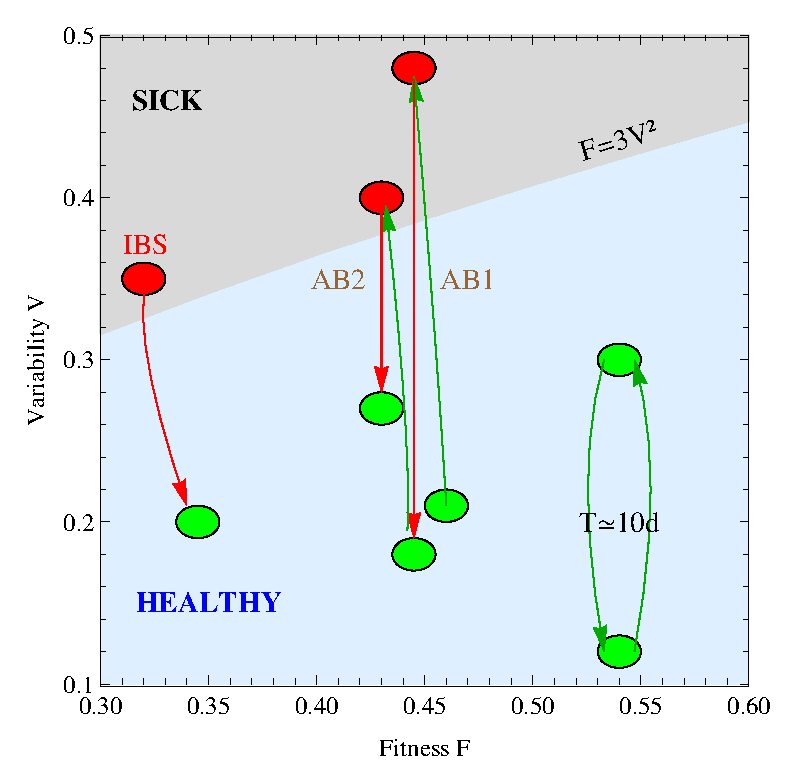
\includegraphics[width=0.8\textwidth]{results/finalPlot33_new.pdf}
	\caption{Microbiota states can be placed in the phase space $F$--$V$. The light blue shaded region corresponds to the stable phase, while the grey shaded region is the unstable phase (the phase transition line is calculated for  $\alpha$ = $\beta$ = 0.75). We place healthy individuals (green) and individuals whose gut microbiota is threatened (antibiotics, IBS) in the phase space fitness--variability. Gut microbiota of healthy individuals over a long term span show a quasi--periodical variability (central period is ten days). We show that taking antibiotics (AB1 and AB2 correspond to first and second treatment respectively) induces a phase transition in the gut microbiota, which impacts its future changes. We also show an IBS--diagnosed patient transiting from the unstable to the stable phase.}
	\label{fig:main3}
\end{figure}

The model predicts two phases for the gut microbiome: a stable phase with large variability that permits some changes in the relative abundances of taxa and an unstable phase with larger variability, above the phase transition, where the order of abundant taxa varies significantly with time. The microbiome of all healthy individuals was found to be in the stable phase, while the microbiome of several other individuals was shown to be in the unstable phase. In particular, individuals taking antibiotics and IBS--diagnosed patient P2 had the most severe symptoms. In this phase diagram, each microbiota state is represented by a point at its measured variability $V$ and inferred fitness $F$. The model predicts high average fitness for all taxa, i.e., taxa are narrowly distributed in F. The fitness parameter has been chosen with different values for demonstrative purposes. Fitness is larger for the healthiest subjects and smaller for the IBS--diagnosed patients.

%%%
\subsection*{Specific results}

\subsubsection*{Fit Plots}
For each and every dataset included in the study, an unweighted fit (see Material and Methods section for details) and a X-weighted fit (detailed in Material and Methods subsection) have been calculated for standard deviations versus the mean values for each bacterial genus monitored in time. Figure \ref{fig:main1} showed the X-weighted fit for samples from a healthy subject (patient A, top) and from a subject diagnosed with irritable bowel syndrome (patient P2, bottom) studied in our lab\cite{IBS}, while Figure \ref{fig:fits} shows the corresponding unweighted fits. Additionally, for the unweighted fit, a complete residues analysis was performed, and a 4-in-1 figure was generated as shown in Figure \ref{fig:unwRes}, corresponding to patient A (top plot in Figure \ref{fig:main1} and Figure \ref{fig:fits}). Among other tests, it allows to check for normality and homoscedasticity of the residues and, therefore, to further evaluate the goodness of the fit.

\begin{figure}
	\centering
	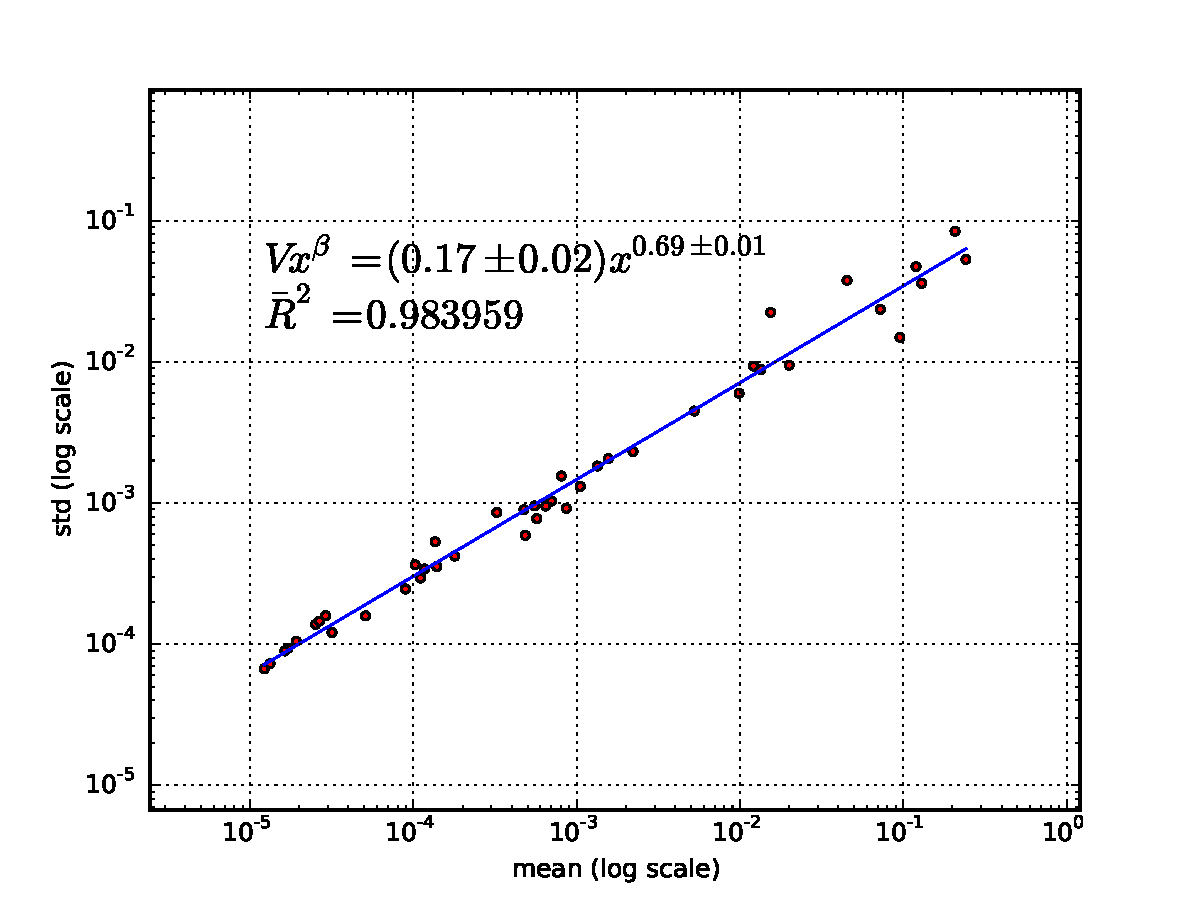
\includegraphics[width=0.8\textwidth]{results/fits/IBS_h_A_amplicons_family_stdVSmean_LLR_LOG.pdf}
	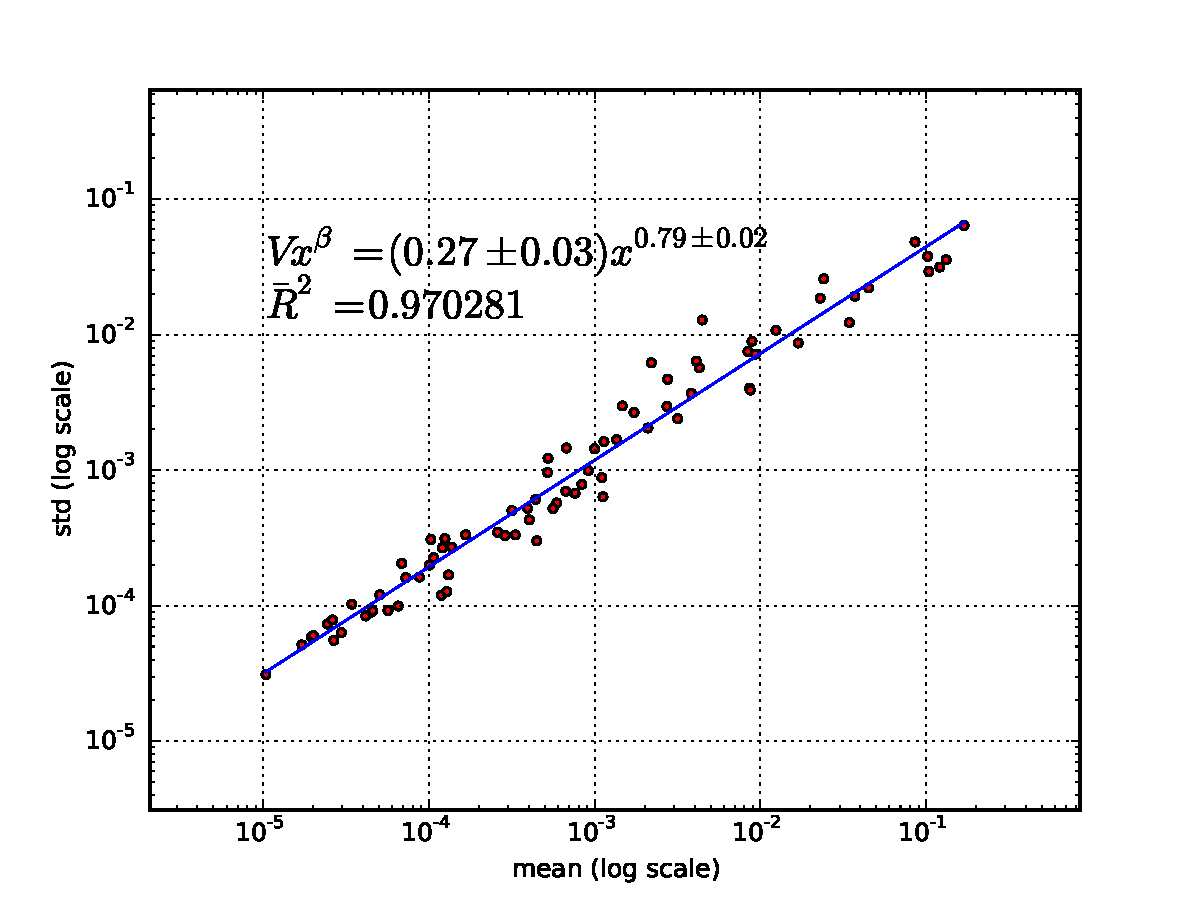
\includegraphics[width=0.8\textwidth]{results/fits/IBS_P1_metatranscriptomes_family_stdVSmean_LLR_LOG.pdf}
	\caption{Log plots of unweighted fits corresponding to the datasets shown in Figure \ref{fig:main1}}
	\label{fig:fits}
\end{figure}

\begin{figure}
	\centering
	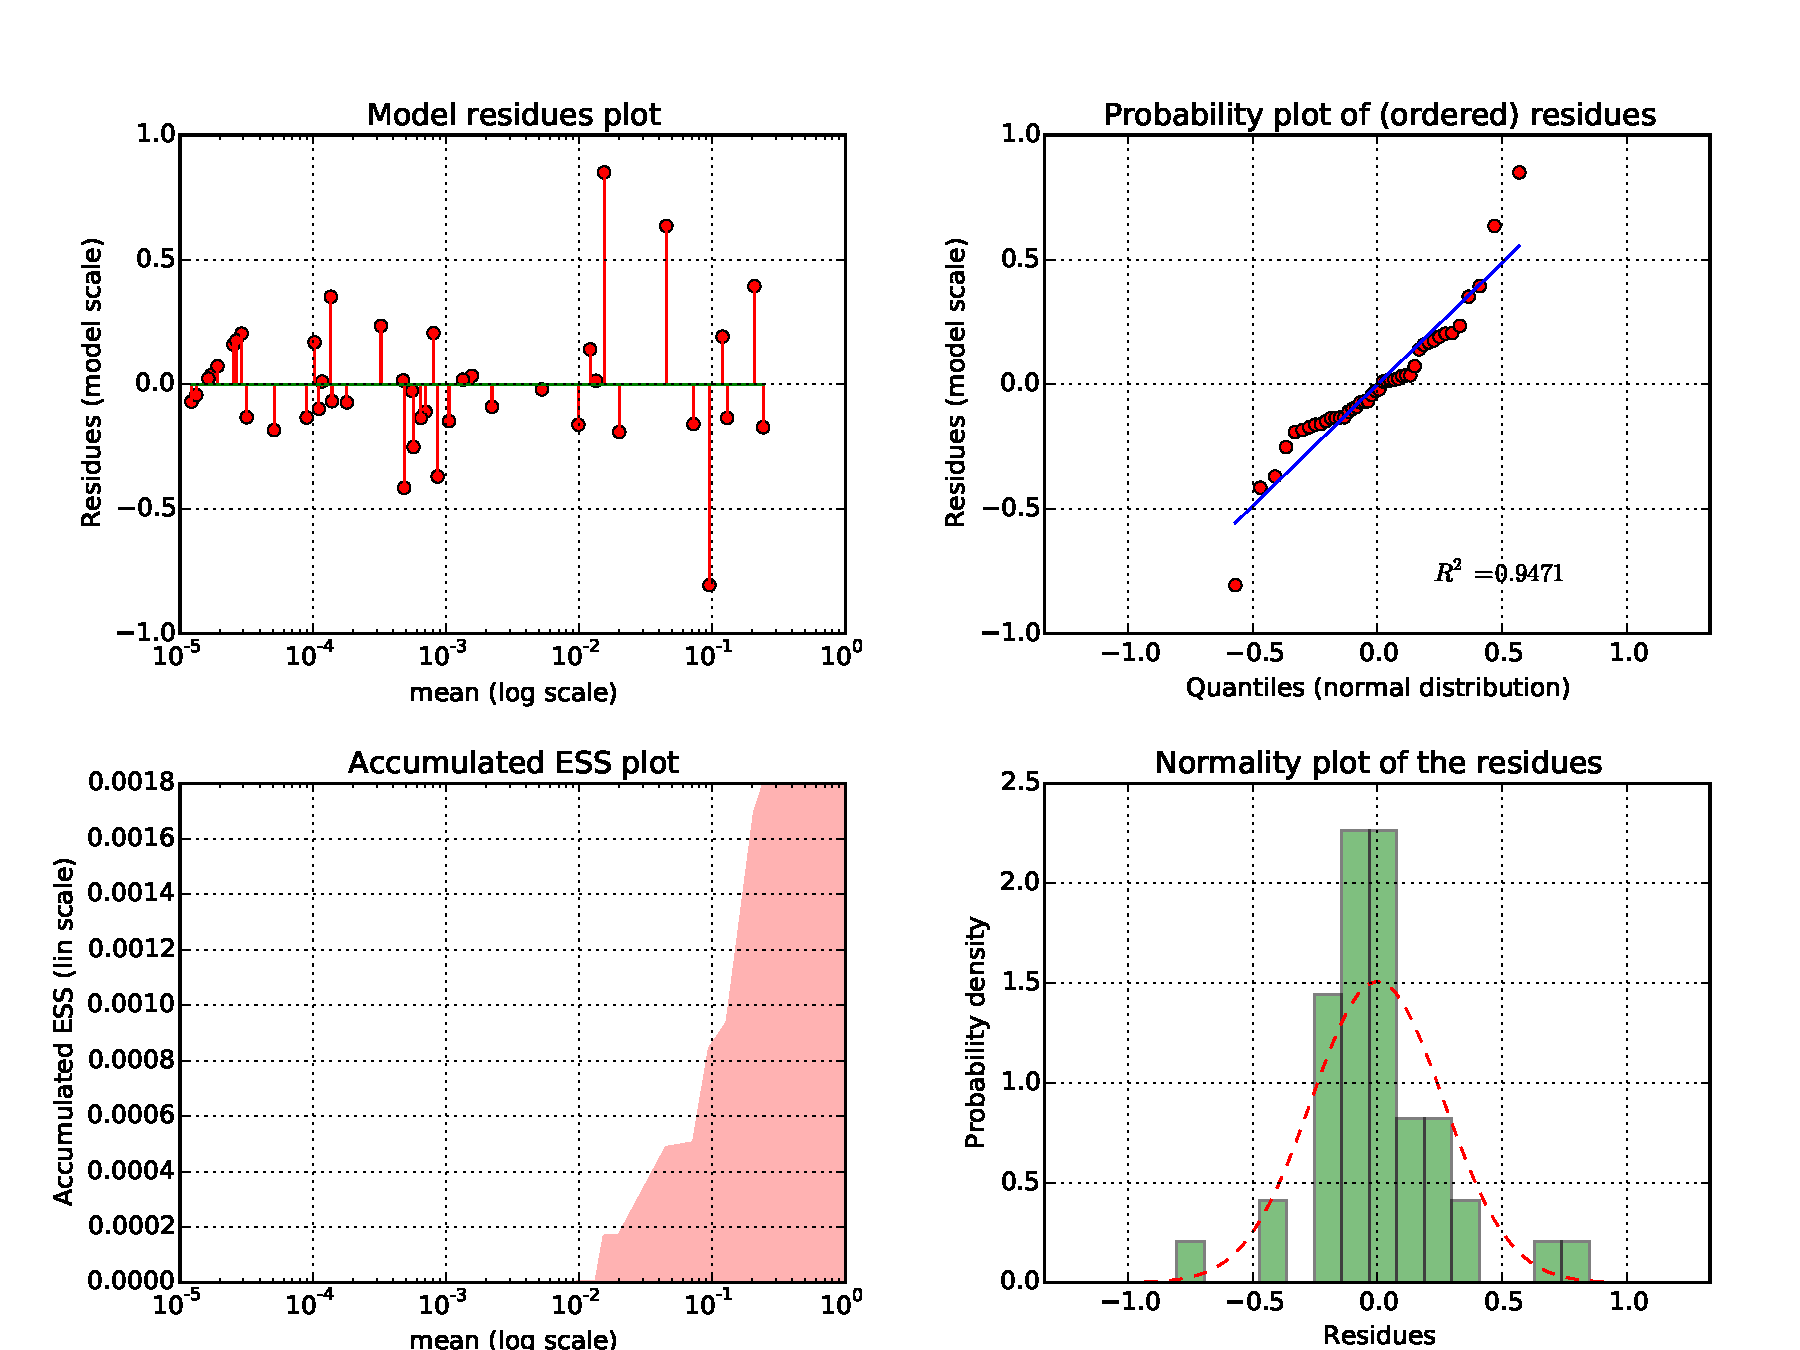
\includegraphics[width=\textwidth]{results/fits/IBS_h_A_amplicons_family_stdVSmean_LLR_RES.pdf}
	\caption{Residues analysis plot corresponding to the unweighted fit for patient A of the IBS study\cite{IBS}. The top-left subplot is a simple residues plot. The top-right subplot is a Normal quantiles plot with linear fitting (value of coefficient of determination is provided). The bottom-left subplot shows an accumulated ESS (Explained Sum of Squares) plot. Finally, the bottom-right subplot is a residues Normal histogram plot. This set of subplots allows to check for normality and homoscedasticity of the residues.}
	\label{fig:unwRes}
\end{figure}

\subsubsection*{Histogram Plots} 
\CC\ generates two related histogram plots, absolute frequencies plot and zero relative frequency plot. The former is useful to visually assess the validity of the time points in terms of the accumulated absolute frequency of the elements (taxa), since absolute frequencies far (much higher or much lower) from those typically observed could mean a sampling problem. In Figure \ref{fig:histAFP} shows this histogram for the pre-treatment data (first 7 times) of patient ``D'' in the antibiotics study\cite{antibiotic}. On the other hand, we could define the ZRF (Zero Relative Frequency, thereby ranging from 0 to 1) of an element (taxon) as the portion of times where it is zero, i.e., it is not found. Attending to all taxa, we can plot the ZRF histogram, which then lies on the horizontal axis of the plot. The vertical axis shows the number of taxa, so the height of a bar represents the amount of taxa that have determinate ZRF. In this respect, the bar over $0.0$ counts the quantity of taxa that are present at every time point of the data set (aka ``core''), while the bar over $1.0$ would count the total of taxa that are never found (this bar never appears because all these ``null'' elements are automatically filtered by the software. Figure \ref{fig:histZRF} shows this plot for the healthy patient A of the IBS study performed in our lab\cite{IBS}. There, we can see that $12$ taxa are present at all the time points of the time series while $9$ taxa basically appear only once. So, this plot is clearly useful to notice how the ``core'' is distributed.
	
\begin{figure}		
	\centering		
 	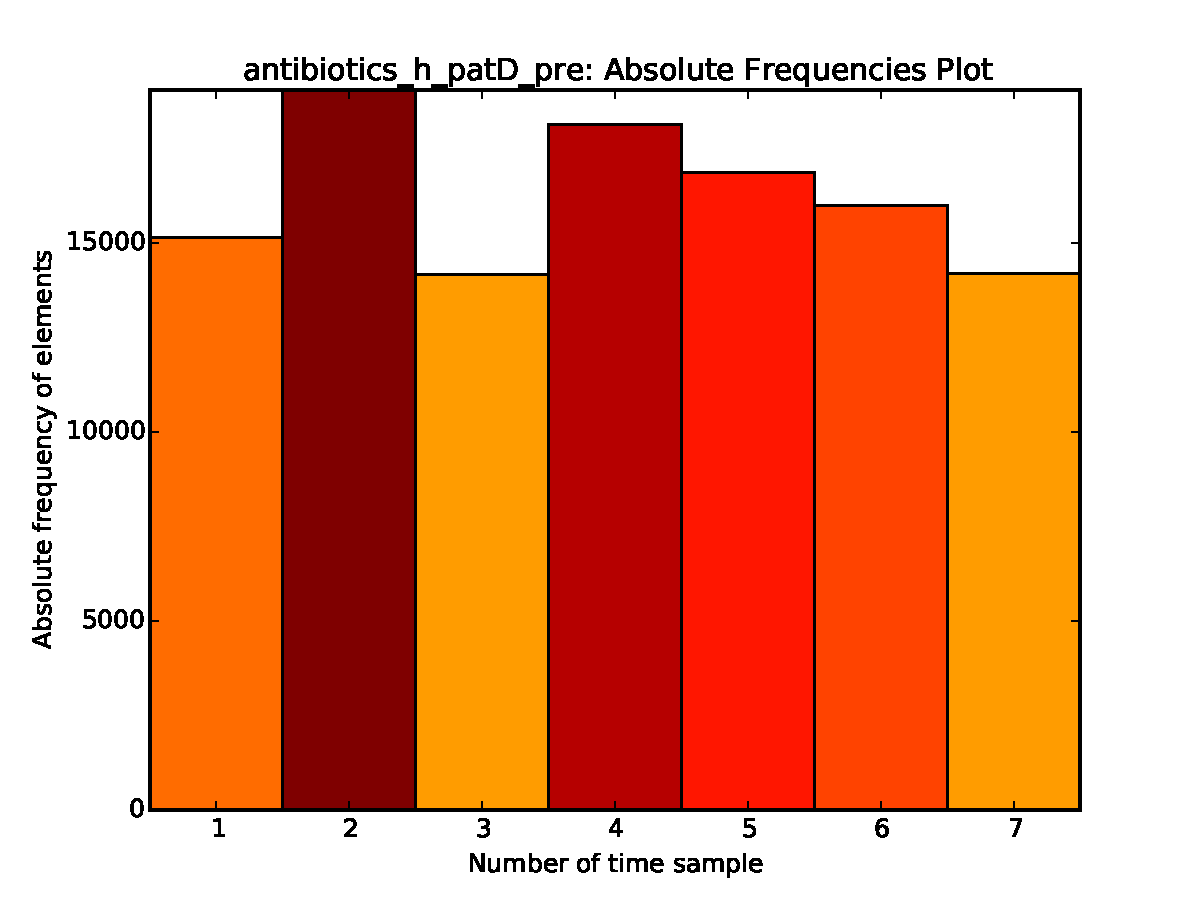
\includegraphics[width=0.8\textwidth]{results/hist/antibiotics_h_patD_pre_AbsFreqPlot}		
 	\caption{Histogram with the absolute frequencies of the pre-treatment data (7 first times) of patient ``D'' in the antibiotics study\cite{antibiotic}. We can see that there are no \emph{outlayers} among the total taxa sum for the time series points, so all of them were considered for further analysis by \CC\ software}		
 	\label{fig:histAFP}		
\end{figure}

\begin{figure}
	\centering
	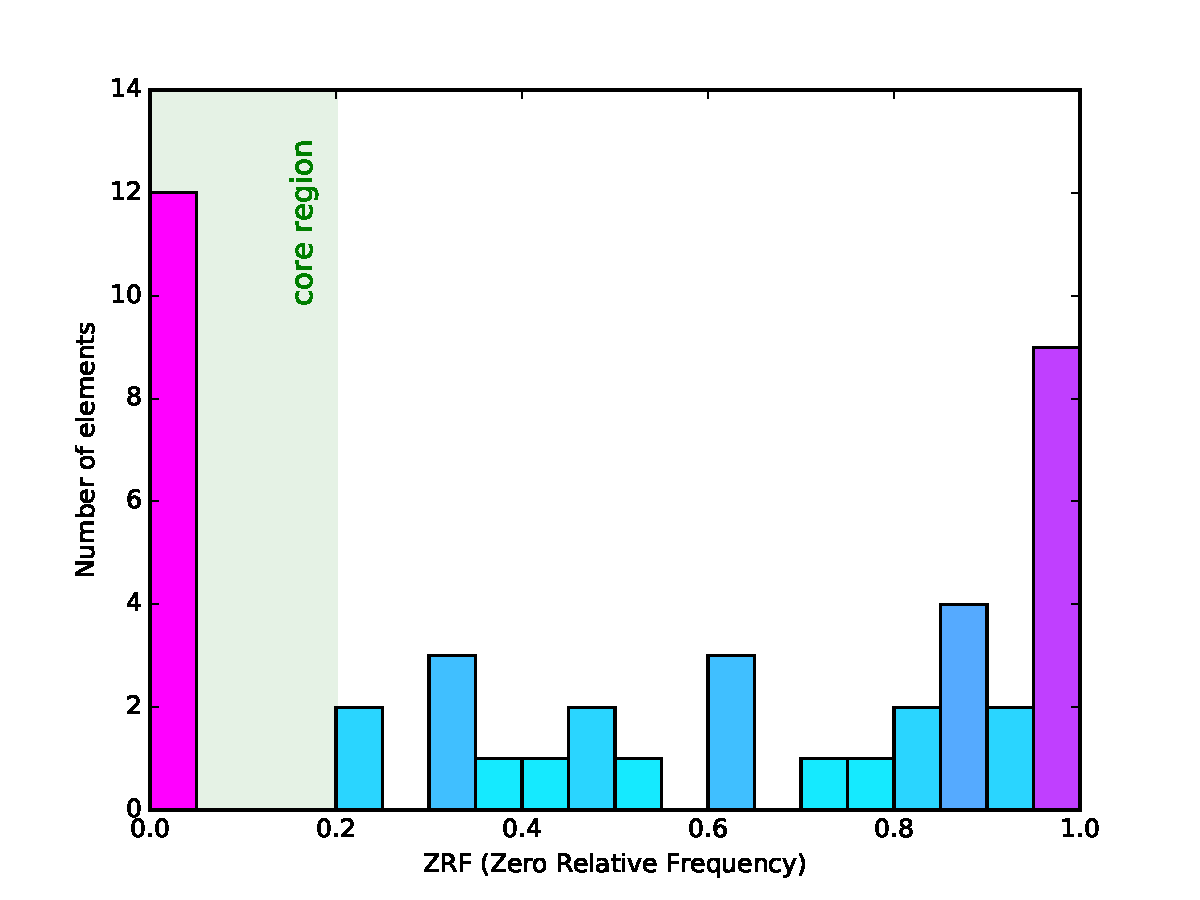
\includegraphics[width=0.8\textwidth]{results/hist/IBS_h_A_amplicons_family_ZRFhist.pdf}
	\caption{Histogram with the relative frequency of zero for the elements (taxa) in the data for patient A of the IBS study\cite{IBS}. In this particular case, the bar over $0.0$ counts the quantity of taxa that are present at every time point of the data set (``core''), while the bar over $1.0$ sums the total of taxa that are never found (this bar never appears because all these ``null'' elements are automatically filtered by \CC): here, $12$ taxa are present at all the time points of the time series while $9$ taxa basically appear only once.}
	\label{fig:histZRF}
\end{figure}

A 2D semi-logarithmic histogram representing deviations from the mean versus the mean itself is a useful tool in the analysis of the stability of ranking processes in complex systems\cite{ranking}. Figure \ref{fig:hist2D} shows this 2D deviation plot for the patient A of the IBS study\cite{IBS}.
 
\begin{figure}
	\centering
	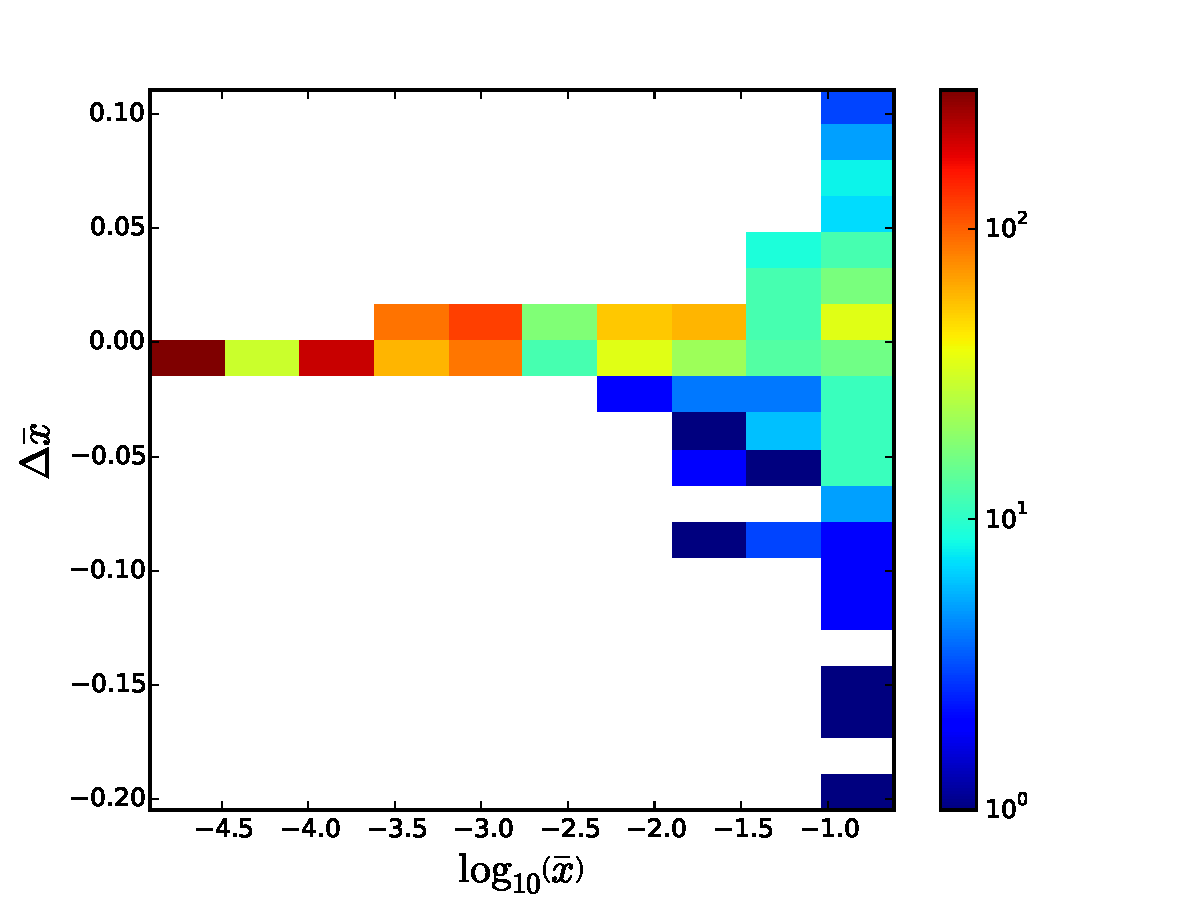
\includegraphics[width=0.8\textwidth]{results/hist/IBS_h_A_amplicons_family_hist2D.pdf}
	\caption{2D histogram deviation plot of the data for patient A of the IBS study\cite{IBS}}
	\label{fig:hist2D}
\end{figure}


\subsubsection*{Correlation and Rank Plots} 
\CC\ generates two different plots falling under this category, as well as Excel files with the resulting matrices. On the one hand, the elements correlation matrix plot shows a correlation matrix among the taxa, calculated with the time as independent variable. For these calculations, the data set is not normalized to avoid entering an additional constraint. Figure \ref{fig:corrElm} shows this matrix for the most dominant taxa present in the data of the patient ``A'' of the IBS study\cite{IBS}. On the other hand, the rank dynamics and stability plot shows the variation in the rank with time for the most dominant taxa and their calculated RSI, as discussed in Material and Methods. Figure \ref{fig:corrank} shows this plot for the taxa of the aforementioned patient A.

\begin{figure}
	\centering
	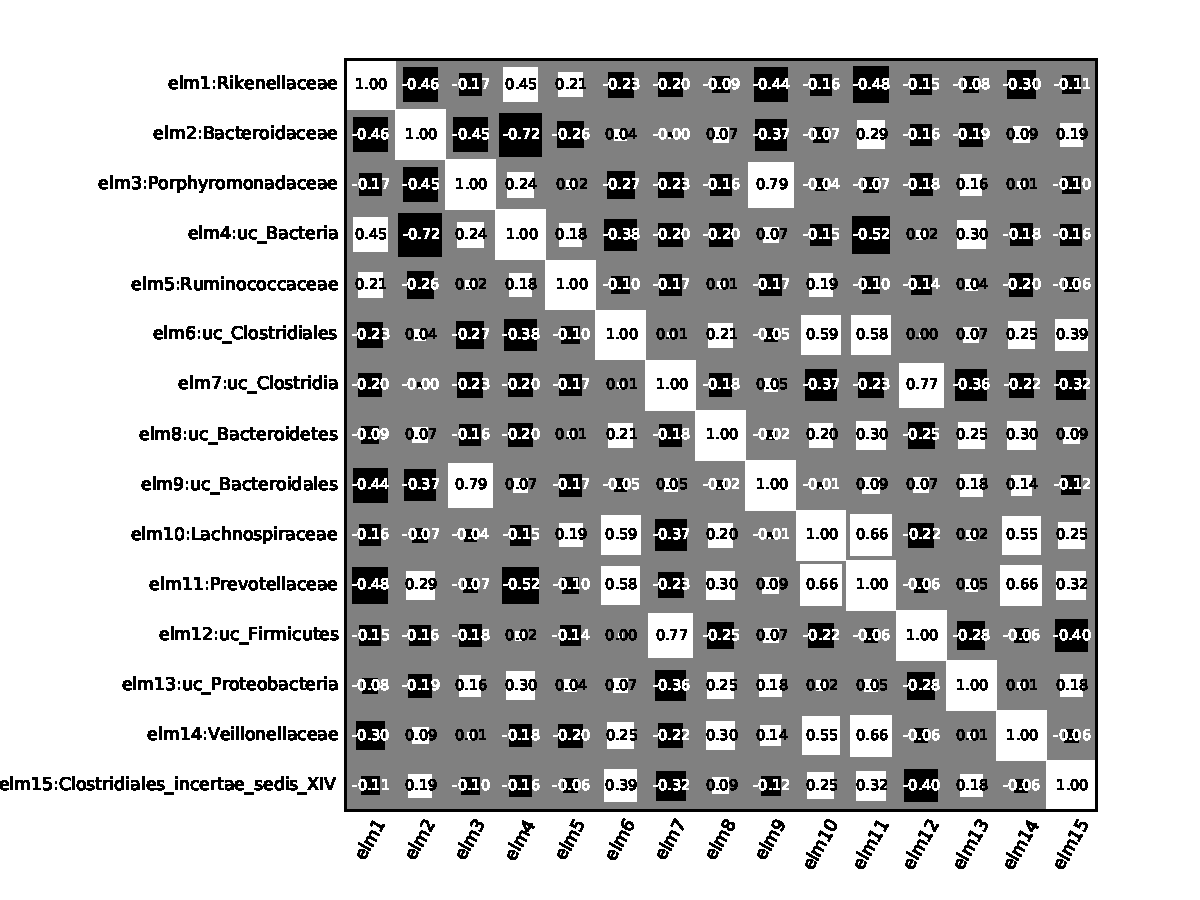
\includegraphics[width=0.9\textwidth]{results/corrank/IBS_h_A_amplicons_family_ElmCorrelation.pdf}
	\caption{Element correlation plot of the for the most dominant taxa in the data for patient A of the IBS study\cite{IBS}}
	\label{fig:corrElm}
\end{figure}

\begin{figure}
	\centering
	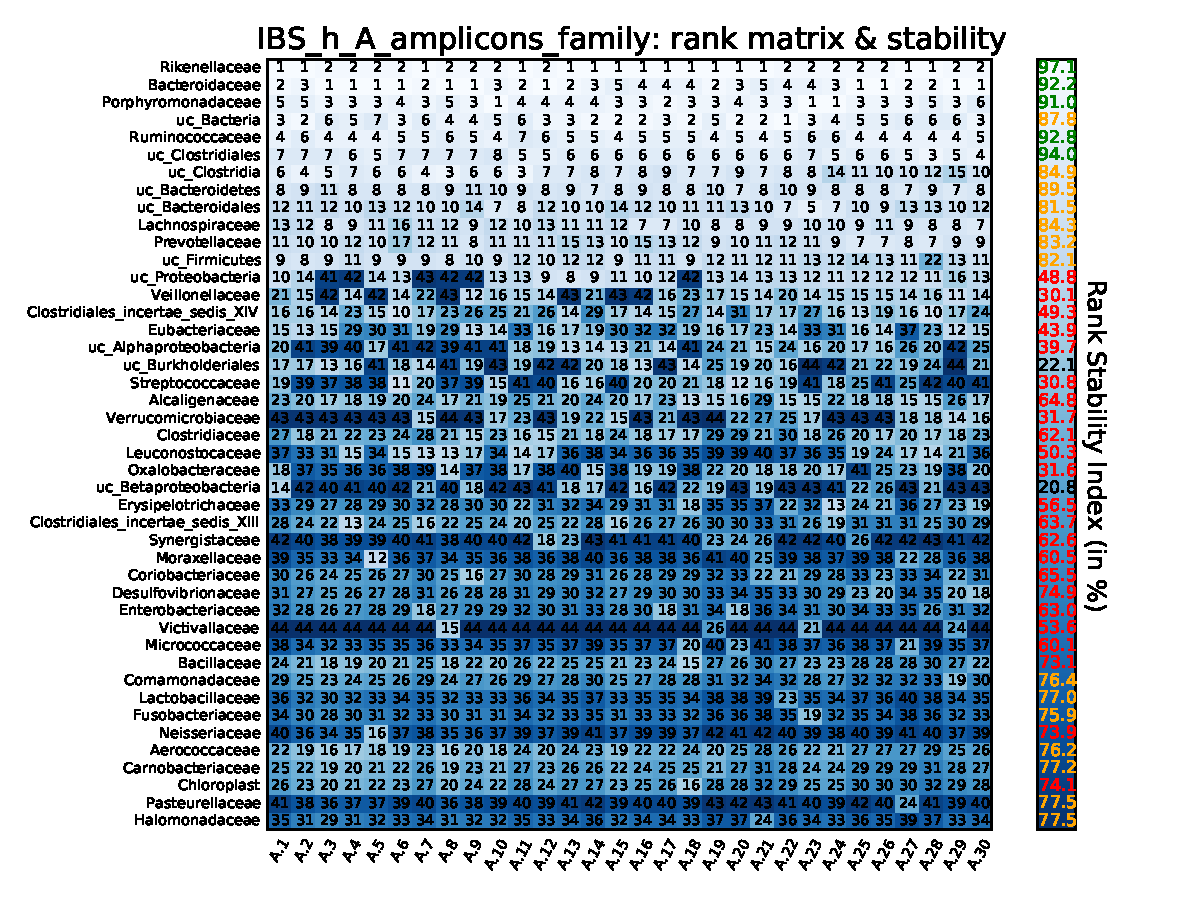
\includegraphics[width=\textwidth]{results/corrank/IBS_h_A_amplicons_family_Rank.pdf}
	\caption{Matrix showing the rank variation throughout time for the most dominant elements (taxa) and their calculated Rank Stability Index (as discussed in Material and Methods) in the data  for patient A of the IBS study\cite{IBS}}
	\label{fig:corrank}
\end{figure}


%%%
\subsection*{Time dependence of model parameters}

Finally, we have studied the time dependence of the variability $V$ and power law index $\beta$ (see Model under Material and Methods) by using a sliding window approach. The total number of time points are divided in subsets of five points, where next subset is defined by adding next time sampling and by eliminating the earliest one. Both parameters were calculated for each subset against the average time lapse. Figure \ref{fig:tempevo1} shows the variability  $V$ as a function of time for the largest sampling: two individuals in the Caporaso's study\cite{moving} corresponding to the gut microbiota of a male (upper plot) and a female (lower plot). Figure \ref{fig:tempevo2} shows the time evolution of $V$ for patient P2 of the IBS study\cite{IBS} (upper plot) and patient D in the antibiotics study\cite{antibiotic} (lower plot). 

\begin{figure}
	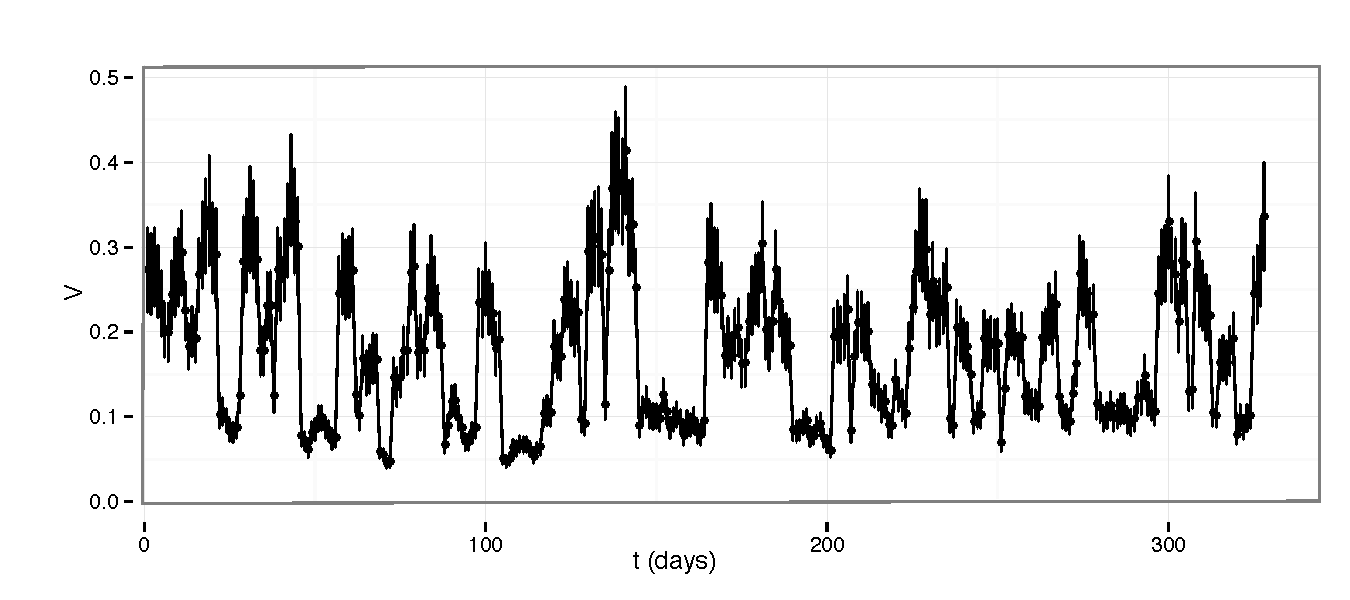
\includegraphics[width=1.0\textwidth]{results/sliwin/male_mov.pdf}
	\hspace*{3mm}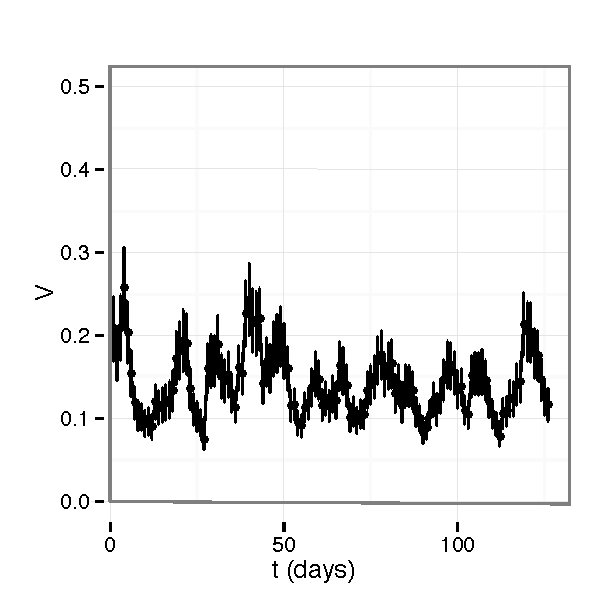
\includegraphics[width=0.448\textwidth]{results/sliwin/female_mov.pdf}
\caption{$V$ as a function of time for the two individuals in the Caporaso's study\cite{moving}: samples of gut microbiome of a male (upper plot) and a female (lower plot). Both samples show changes in the variability V with quasi--periodic behavior peaked at about 10 days. Variability grows more for the gut microbiota of the male and share a minimal value around 0.1 with the gut microbiota of the female.}
\label{fig:tempevo1}
\end{figure}

\begin{figure}
	\centering 
 	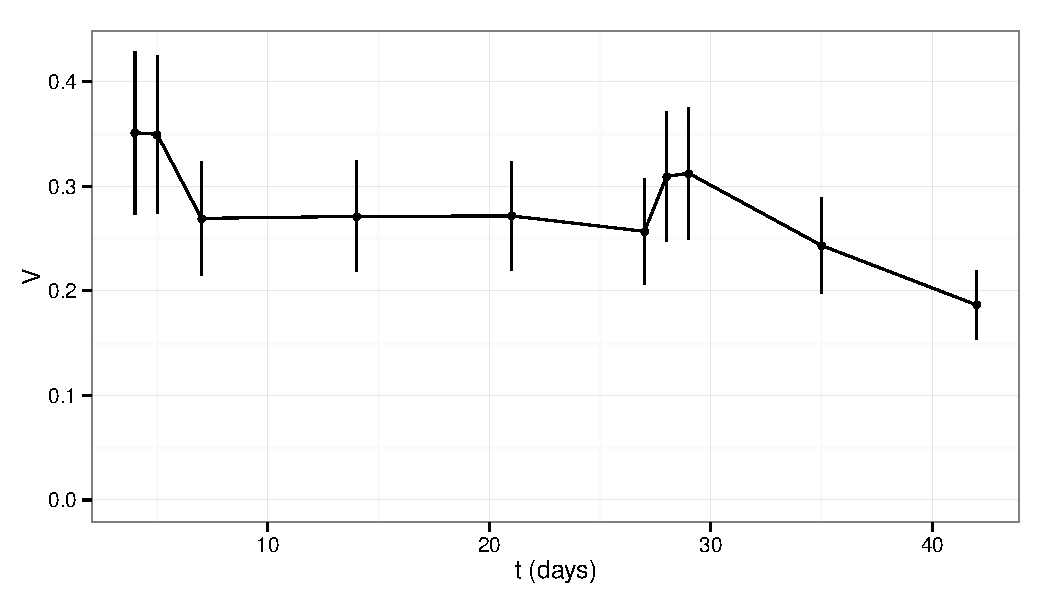
\includegraphics[width=0.8\textwidth]{results/sliwin/patP2_IBS.pdf}
  	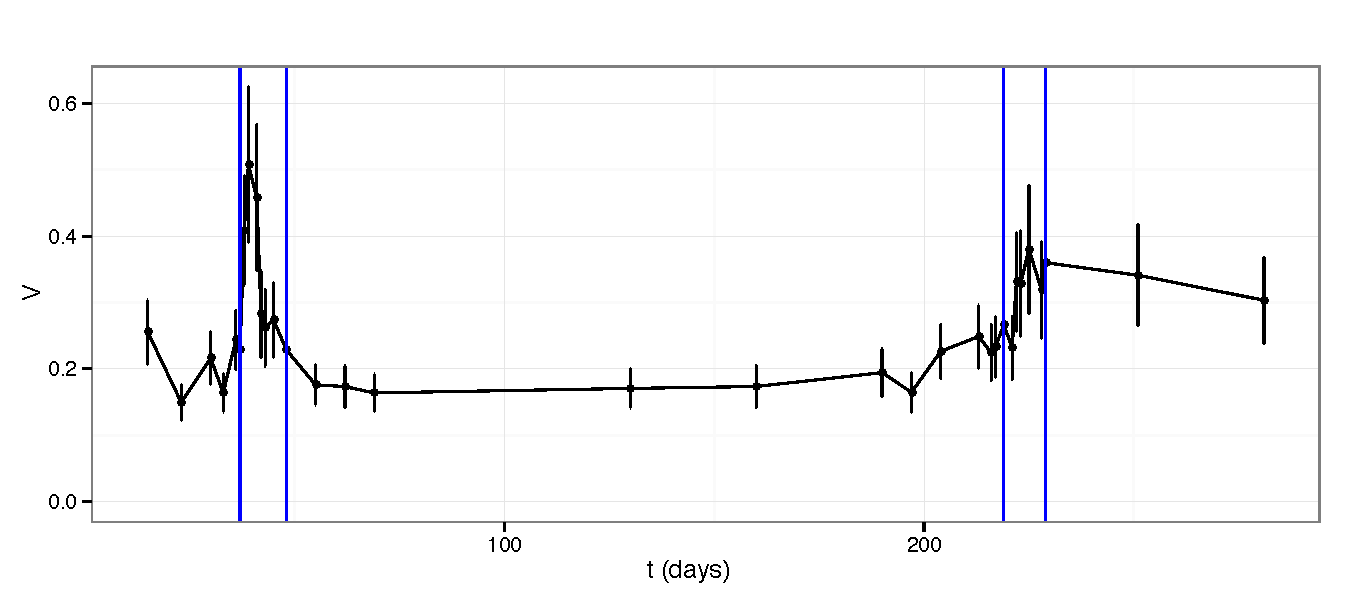
\includegraphics[width=1.0\textwidth]{results/sliwin/patD_antibio.pdf} 
\caption{$V$ as a function of time for patient P2 of the IBS study\cite{IBS} (upper plot) and patient D in the antibiotics study\cite{antibiotic} (lower plot). The variability 
of the gut microbiota of P2 decreases from above 0.3 to below 0.2, showing a slow tendency to increase the order of the system.  Antibiotic intake leaks to a quick increase of variability which lasts for a few days to recover ordering. The second antibiotic treatment shows some memory (lower increase of variability) with a slower recovery. NOTE: The blue vertical lines in the lower plot are showing the periods of antibiotic treatment.}
\label{fig:tempevo2}
\end{figure}
